\documentclass[parskip=full]{scrartcl}
\usepackage[T1]{fontenc}    % avoid garbled Unicode text in pdf
\usepackage[utf8]{inputenc} % use utf8 file encoding for TeX sources
\usepackage[german]{babel}  % german hyphenation, quotes, etc
\usepackage{hyperref}       % detailed hyperlink/pdf configuration
\hypersetup{                % ‘texdoc hyperref‘ for options
pdftitle={PSE: Entwicklung eines relationalen Debuggers - Pflichtenheft},%
,%
}
\usepackage{graphicx}       % provides commands for including figures
\usepackage{csquotes}       % provides \enquote{} macro for "quotes"
\usepackage[nonumberlist]{glossaries}     % provides glossary commands
\usepackage{enumitem}
\usepackage{xcolor}
\newcommand\frage[1]{\textcolor{red}{#1}}


\newglossaryentry{Debugger}
{
	name={Debugger},
	description={Ein Debugger ist ein Werkzeug zum Diagnostizieren und Auffinden von Fehlern in Computerprogrammen}
}
\newglossaryentry{Variableninspektor}
{
	name={Variableninspektor},
	plural={Variableninspektoren},
	description={Zeigt die Variablen des Programms und deren Belegung an}
}
\newglossaryentry{Relationale Eigenschaft}
{
	name={Relationale Eigenschaft},
	plural={Relationale Eigenschaften},
	description={}%TODO
}
\newglossaryentry{Interpreter}
{
	name={Interpreter},
	description={Teil des Produkts, welches die definierte Sprache ausführt}
}
\newglossaryentry{Tooltip}
{
	name={Tooltip},
	plural={Tooltips},
	description={Zeigt eine Beschreibung zu einem Element der Benutzeroberfläche}
}

\newglossaryentry{Einzelschritt}
{
	name={Einzelschritt},
	plural={Einzelschritte},
	description={Ein Einzelschritt entspricht einem ausgeführten Befehl}
}
\newglossaryentry{Schritt}
{
  name={Schritt},
  plural={Schritte},
  description={Siehe Einzelschritt. Die Anzahl ausgeführter Befehle entspricht der Schrittgröße}
}
\newglossaryentry{Step-Out}
{
	name={Step-Out},
	description={Springt bis zum Ende der aktuell ausgeführten Funktion. Befindet sich der Debugger in der main-Funktion, wird das Programm fertig gedebuggt}
}
\newglossaryentry{Step-Over}
{
	name={Step-Over},
	description={Ist der Befehl in der aktuellen Zeile ein Methodenaufruf, wird das Programm bis zum Ende dieser Methode gedebuggt. Ist der Befehl eine einzelne Ausführung,
	wird diese wie bei einem Einzelschritt ausgeführt}
}
\newglossaryentry{Breakpoint}
{
	name={Breakpoint},
	plural={Breakpoints},
	description={Erreicht das Produkt einen Breakpoint, stoppt es an dieser Stelle das Debuggen}
}
\newglossaryentry{bedingter Breakpoint}
{
	name={bedingter Breakpoint},
	plural={bedingte Breakpoints},
	user1={bedingten Breakpoints},
	user2={Bedingte Breakpoints},
	description={Der Benutzer kann Relationen zwischen Variablen der zu debuggenden Programme angeben. Sobald diese Relation zutrifft, stoppt das Produkt das Debuggen,
	auch wenn aktuell ein Schritt ausgeführt wird, der weiter springen würde. Weiteres dazu ist in Kapitel 12 zu finden}
}
\newglossaryentry{Watch-Expression}
{
	name={Watch-Expression},
	plural={Watch-Expressions},
	description={Der Benutzer kann Ausdrücke, die sich auf Variablen in den zu debuggenden Programmen beziehen, als Watch-Expressions angeben. Er wird dann beim Debuggen dauerhaft über den aktuellen Zustand des ausgewerteten Ausdrucks informiert. Weiteres dazu ist in Kapitel 12 zu finden}
}
\newglossaryentry{Debugmodus}
{
	name={Debugmodus},
	description={Das Produkt befindet sich im Debugmodus, sobald der Benutzer Start auswählt. Im Debugmodus können Eingabevariablen und die zu debuggenden Programme nicht
	mehr geändert werden}
}
\newglossaryentry{Editiermodus}
{
	name={Editiermodus},
	description={Das Produkt befindet sich im Editiermodus, bevor der Benutzer den Debugmodus startet, und nachdem das Debuggen abgeschlossen ist. Im Editiermodus
	können Eingabevariablen und die zu debuggenden Programme geändert werden}
}
\newglossaryentry{Konfigurationsdatei}
{
	name={Konfigurationsdatei},
	plural={Konfigurationsdateien},
	description={Der Benutzer kann Konfigurationsdateien bezüglich eines Durchlaufs des Produkts erstellen. Diese Dateien enthalten die zu debuggenden Programme,
	Breakpoints, Watch-Expressions, Eingabevariablen, Schrittgrößen und die Stelle, an der das Debuggen eventuell unterbrochen wurde}
}



\let\glsplgen\glsuseri
\let\glsplcap\glsuserii

\makeglossaries

\title{
	\vspace{2cm}
	PSE:\\ 
	Entwicklung eines relationalen Debuggers\\
}
\subtitle{
	\vspace{1cm}Pflichtenheft
}
\author{
	\vspace{1cm} \\
	Benedikt Wagner\\
	\texttt{udpto@student.kit.edu}
	\and \vspace{1cm} \\ Chiara Staudenmaier\\
	\texttt{uzhtd@student.kit.edu}
	\and Etienne Brunner\\
	\texttt{urmlp@student.kit.edu}
	\and Joana Plewnia\\
	\texttt{uhfpm@student.kit.edu} 
	\and Pascal Zwick\\
	\texttt{uyqpk@student.kit.edu}
	\and Ulla Scheler\\
	\texttt{ujuhe@student.kit.edu}
}


\begin{document}

\maketitle
\newpage

\tableofcontents
\newpage

%Eventuell Fußnoten generieren

\section{Produktübersicht}
%kurze Übersicht über das Produkt
Das Produkt \enquote{DIbugger} soll dem Nutzer die Möglichkeit bieten, mehr als ein Programm gleichzeitig zu debuggen und interaktiv zu analysieren. \\
Dabei sollen die Konzepte eines herkömmlichen Debuggers, namentlich \glspl{Einzelschritt}, \glspl{Breakpoint} und Variableninspektion, erhalten bleiben und um zusätzliche Konzepte, die den Umgang mit zwei oder mehr Programmläufen erleichtern, erweitert werden. Zu diesen Konzepten gehören das betrachten von sogenannten \glspl{Watch-Expression}, bei denen der Nutzer beispielsweise Differenz oder Quotient aus zwei Variablen aus den verschiedenen Programmen untersuchen kann. Der Fokus liegt hierbei auf der Unterstützung des Findens von relationalen Zusammenhängen in den vom Nutzer in einer WHILE-Sprache, welche eine Teilmenge von Java darstellt und in Kapitel 12 näher definiert wird, verfassten Programmen.
\vspace{1cm}
\begin{figure}[!h]
\centering

\includegraphics[width=0.85\textwidth]{logo_nongi.png}
\caption{Produktlogo}
\end{figure}
\newpage

\section{Produkteinsatz}
Das Produkt unterstützt das Institut für theoretische Informatik am Karlsruher Institut für Technologie beim Führen von Beweisen zu relationalen Eigenschaften von Programmen. Hierbei soll die Möglichkeit des gleichzeitigen Debuggens der Programme dem Nutzer bei der Beweisführung helfen. \\
Verwendet wird das Produkt hierbei von wissenschaftlichen Mitarbeitern am Lehrstuhl ''Anwendungsorientierte formale Verifikation - Prof. Dr. Beckert'' des Instituts für theoretische Informatik am Karlsruher Institut für Technologie und soll in deren Büroumgebung zum Einsatz kommen. 

%Anwendungsbereiche, Zielgruppen, Betriebsbedingungen
 

\section{Produktumgebung}
%Software, Hardware, Orgware, Schnittstellen
Das Produkt läuft auf dem Rechner des Nutzers und benötigt keine Kommunikation mit außerhalb. Hierbei läuft das Produkt eventuell neben anderen Applikationen, kommuniziert jedoch nicht mit diesen.

\subsection{Software}
Da es sich bei dem Produkt um ein Java-Programm handelt, muss ein JRE (Java Runtime Environment) der Version 8 oder höher auf dem Rechner vorhanden sein oder mitinstalliert werden. \\
Das Produkt läuft sowohl auf Windows, als auch auf Mac OS und Linux (64bit empfohlen).

\subsection{Hardware}
An die Hardware des Rechners werden keine speziellen Anforderungen gestellt. Das Produkt läuft auf Rechnern mit mindestens einem 1 GHz Prozessor und 1 GB RAM.

\subsection{Schnittstellen}
Das Produkt hat Schnittstellen zur graphischen Benutzeroberfläche und zum Interpreter, um diese leicht austauschbar zu gestalten. \\
Außerdem können durch eine öffentliche Schnittstellen, mittels austauschbarer Sprachkonfigurationsdateien, verschiedene Sprachen der Benutzeroberfläche genutzt werden. 

\newpage

\section{Produktfuntionen}
	 	\subsection{Funktionale Anforderungen}
 		\subsubsection{Musskriterien}
		\begin{itemize}
		\item[/FA10/] Das Produkt ist ein Debugger für Quelltexte, welche in der im Kapitel Ergänzungen spezifizierten Sprache geschrieben sind.
		\item[/FA20/] Im Debugmodus kann der Benutzer \glspl{Schritt} (Steps) durchführen.
		\item[/FA30/] Es ist möglich, von den anderen Programmen unabhängige \glspl{Einzelschritt} in einem Programm auszuführen.
		\item[/FA40/] Der Benutzer kann die Schrittgröße für jedes Programm einzeln festlegen.
		\item[/FA50/] Bei einem \gls{Schritt} wird die vorgegebene Anzahl an Befehlen ausgeführt. Dabei werden die Befehle einer Funktion einzeln ausgeführt (automatisches Step-In). 
		\item[/FA60/] Der Benutzer kann durch \gls{Step-Out} eine Funktion verlassen.
		\item[/FA70/] Durch \gls{Step-Over} kann eine Funktion als einzelner auszuführender Befehl abgearbeitet werden.
		\item[/FA80/] Der Benutzer kann \glspl{Breakpoint} an Zeilen im Quelltext setzen.
		\item[/FA90/] Der Benutzer kann relationale Eigenschaften bezüglich Variablen als \glspl{bedingter Breakpoint} festlegen.
		\item[/FA100/] \glspl{bedingter Breakpoint} können an vom Benutzer bestimmte Stellen im Quelltext gebunden werden.
		\item[/FA110/] Der Benutzer kann relationale Eigenschaften bezüglich Variablen als \glspl{Watch-Expression} festlegen.
		\item[/FA120/] \glspl{Watch-Expression} können an vom Benutzer bestimmte Stellen im Quelltext gebunden werden.
		\item[/FA130/] Im \gls{Debugmodus} kann der Benutzer durch Auswahl der Option Weiter das Programm bis zum nächsten Breakpoint debuggen.
		\item[/FA140/] Das Produkt bietet die Möglichkeit, eine \gls{Konfigurationsdatei} für einen Lauf zu speichern. Diese beinhaltet festgelegte Eingabewerte, Breakpoints, Watch-Expressions, Schrittgröße und die zu debuggenden Quelltexte.
		\item[/FA150/] Das zu debuggende Programm kann direkt in die Textbox des Produkts  geschrieben werden.
		\item[/FA160/] Das zu debuggende Programm kann direkt in die Textbox des Produkts kopiert werden.
		\item[/FA170/] Das zu debuggende Programm kann aus einer Textdatei eingebunden werden.
		\item[/FA180/] Der \gls{Debugmodus} kann vom Benutzer abgebrochen werden. Dadurch kehrt der Benutzer zum \gls{Editiermodus} zurück.
		\item[/FA190/] Nach jedem Schritt oder \gls{Breakpoint} werden die aktuellen Variablenbelegungen angezeigt.
		\item[/FA200/] Die Variablenreihenfolge im Variableninspektor ist manuell veränderbar.
		\item[/FA210/] Im Variableninspektor können Variablen ausgeblendet werden.
		\item[/FA215/] Das Produkt ermöglicht die automatische Generierung von fehlenden Benutzerangaben für Eingabewerte.
		\end{itemize}

 		\subsubsection{Sollkriterien}
		\begin{itemize}
		\item[/FA220/] Das Produkt kann zufällige Vorschläge für Eingabewerte über einen Vorschlag-Button erstellen. Der Benutzer kann diese noch ändern.
		\item[/FA230/] Der Benutzer kann Variablen auswählen, von welchen jeder angenommene Wert gespeichert wird.
		\item[/FA240/] Bei Endlosschleifen wird automatisch abgebrochen. Die maximale Anzahl an Schleifendurchläufe kann vom Benutzer festgelegt werden (maximal 250).
		\item[/FA250/] Der Benutzer kann mehr als zwei Programme simultan debuggen.
		\item[/FA260/] Das Produkt kann Vorschläge für Eingabevariablen anhand der zu debuggenden Programme machen.
		\item[/FA270/] Das Produkt kann Vorschläge für \glspl{Watch-Expression} anhand der zu debuggenden Programme machen.
		\item[/FA280/] Das Produkt kann Vorschläge für \glspl{bedingter Breakpoint} anhand der zu debuggenden Programme machen.
		\end{itemize}

 		\subsubsection{Kannkriterien}
		\begin{itemize}
		\item[/FA290/] Die Datei des zu debuggenden Programms kann in das Textfeld hineingezogen werden.
		\item[/FA300/] Das Produkt kann, abhängig von der Zeilenanzahl der Programme, dem Benutzer die Schrittgröße(Step-Size) vorschlagen.
		\item[/FA310/] Der Benutzer kann Variablen angeben, für welche das Produkt eine Relation vorschlägt.
		\item[/FA320/] Der Benutzer kann einen Rückschritt durchführen.
		\item[/FA330/] Die, an den Quelltext gebundenen, \glspl{Breakpoint} verschieben sich mit dem Quelltext, wenn dieser im \gls{Editiermodus} geändert wird.
		\end{itemize}		 		
 		
 		
 		\subsubsection{Abgrenzungskriterien}
 		\begin{itemize}
 		\item[/A10/] Das Produkt ist auf zu debuggende Programme mit maximal 100 Zeilen Quelltext optimiert. Mehr als 250 Zeilen Quelltext sind nicht zugelassen.
 		\item[/A20/] Das Produkt ist auf zu debuggende Programme mit maximal 100 Iterationen pro Schleife bzw. 100 Rekursionsaufrufe pro Funktion optimiert.
 		\item[/A30/] Das Produkt vergleicht nur Programme die in einem gemeinsamen Durchlauf gedebuggt wurden.
 		\item[/A40/] Das Produkt unterstützt eine maximale Zeilenbreite von 120 Zeichen.
 		\item[/A50/] Das Produkt ersetzt keinen Text-Editor. So hat es zum Beispiel kein Syntax-Highlighting und keine Auto-Vervollständigung.
 		\item[/A50/] Das Produkt ersetzt keine Versionskontrolle. Die Nutzerin ist selbst dafür verantwortlich, ihre Änderungen - zum Beispiel durch Kommentare - zu dokumentieren.
 		\end{itemize}
 		
 \newpage		
 		
	\subsection{Nichtfunktionale Anforderungen}
		\subsubsection{Produktdaten}
		\begin{itemize}
		
		
			\item[/PD10/] Konfigurationsdateien: \\
			Diese Dateien speichern eine Konfiguration des Debuggers. 
			Zu diesen gehören die Eingabewerte, Schrittgrößen, Variablenauswahl, Quelltext und Position beider Programme, aber nicht die Ausgabewerte. \\
			Weiter müssen alle Breakpoints gespeichert werden. Dazu zählen sowohl gesetzte als auch bedingte Breakpoints. Bedingte Breakpoints benötigen keine Speicherung der Zeile, 			sondern die Speicherung eines Bereiches, zweier Variablen der Programmtexte und eines Operators. Dies gilt auch für die Watch-Expressions.
			Zudem wird, falls die Datei aus dem Debugmodus erzeugt wurde, der letzte Status aller Programme gespeichert, um diese nach späterem Laden weiter ausführen lassen zu können. 
			
			\item[/PD20/] Sprachdateien: \\
			Diese Datei speichert die Übersetzung der gesamten Benutzeroberfläche.
			Dazu gehören die Texte der GUI-Elemente und Tooltips.
			
			\item[/PD30/] Einstellungsdatei: \\
			Diese Datei speichert die zuletzt ausgewählte Sprache und die Adresse der Konfigurationsdatei, welche zur zuletzt verwendeten Konfiguration passt.
			
			\end{itemize}
			
			 
		\subsubsection{Produktleistungen}
		%Zeitverhalten, Genauigkeit, Fehlertoleranz
		\begin{itemize}
		\item[/PL10/] Zeitverhalten: \\
		Das Produkt ermöglicht das Hinzufügen von Eingabevariablen, Watch-Expressions, Schrittgröße und Breakpoints in Echtzeit. Das Ausführen von Schritten, Step-Over und Step-Out, sowie das Erreichen des nächsten Breakpoints, ist ebenfalls in Echtzeit möglich. \\
		Den Debugmodus zu starten dauert unter 5 Sekunden. 
		% Kann man das so lassen? Oder dauert Trace-Generierung länger?
		% Pop-Up mit "Trace wird generiert. Dies kann einen Moment dauern"
		\item[/PL20/] Genauigkeit: \\
		Da das Produkt alle primitiven Datentypen von Java unterstützt, ergibt sich für die vom Produkt angezeigten Variablenbelegungen die selbe Genauigkeit wie bei der Ausführung durch die JVM (Java Virtual Machine).
		\newpage
		\item[/PL30/] Fehlertoleranz: \\
		Durch automatisches Ablehnen kritischer Eingaben (A10, A20, A40) und Überprüfung der Semantik, ergibt sich eine hohe Fehlertoleranz bezüglich Benutzereingaben.
		Durch die automatische Generierung von fehlenden Benutzerangaben für Eingabewerte (FA215), wird der Start des Debugmodus zu jeder Zeit ermöglicht.
		\end{itemize}
		
		\subsubsection{Weitere nichtfunktionale Anforderungen}
		%Benutzbarkeit, Wartbarkeit, Erweiterbarkeit, Gesetze/Normen/Sicherheit/Urheberrecht, Robustheit
		\begin{itemize}
		\item[/NA10/]Erweiterbarkeit: \\
		Das Produkt ist, durch seinen modularen Entwurf, erweiterbar um zusätzliche Sprachen für die Benutzeroberfläche, sowie einen Interpreter für weitere Sprachen.
		\item[/NA20/]Wartbarkeit: \\
		Durch seinen Modularen Entwurf, können Fehler, die z.B. durch veraltete Module entstehen, leicht beseitigt werden.
		%\item[/NA25/]Robustheit: \\
		%weiß hier jemand was?
		\item[/NA30/]Urheberrecht: \\
		Das Produkt wird unter Open Source Lizenz entwickelt. Bei der Entwicklung wird das unter BSD-Lizenz veröffentlichte Antlr\textsuperscript{\textcopyright} verwendet.
		Außerdem wird das Produkt in Java entwickelt, welches unter der GNU General Public Lizenz verfügbar ist.
		\item[/NA40/] Sicherheit: \\
		Da das Produkt keine Netzwerkverbindung besitzt, verbleiben die vom Benutzer eingegebenen Daten ausschließlich auf dem Rechner des Benutzers.
		\item[/NA50/]Benutzerfreundlichkeit: \\
		Durch das Hilfemenü werden dem Benutzer die wichtigsten Funktionen und deren Anwendung des Produkts erklärt. Erklärungen zu Bestandteilen der Benutzeroberfläche sind durch \glspl{Tooltip} abgedeckt. \\
		Durch die strikte Trennung der verschiedenen und Gruppierung der zusammengehörigen Elemente der Benutzeroberfläche ergibt sich ein übersichtliches Erscheinungsbild. 
		\end{itemize}
		

\section{Qualitätsanforderungen}
 \begin{tabular}{l||c|c|c|c} 
  Produktqualität & Sehr gut & Gut & Normal & Nicht relevant \\
  \hline
  \hline
  \textbf{Funktionalität} & &&&\\
  Angemessenheit & & & X &  \\
  Richtigkeit & X & & & \\
  Interoperabilität & & & X &\\
  Sicherheit & & & X & \\
  \hline
  \textbf{Zuverlässigkeit} &&&&\\
  Reife & & & X & \\
  Fehlertoleranz & & & X & \\
  Wiederherstellbarkeit & & & X &\\
  \hline
  \textbf{Benutzbarkeit} &&&&\\
  Verständlichkeit & & X & &\\
  Erlernbarkeit & & X & &\\
  Bedienbarkeit & X & & &\\
  \hline
  \textbf{Effizienz} &&&&\\
  Zeitverhalten & & & X & \\
  Verbauchsverhalten & & & X & \\
  \hline
  \textbf{Änderbarkeit} &&&&\\
  Analysierbarkeit & & & X &\\
  Modifizierbarkeit & X & & &\\
  Stabilität & & X&  &\\
  Prüfbarkeit & & & X &\\
  \hline
  \textbf{Übertragbarkeit} &&&&\\
  Anpassbarkeit & & X & &\\
  Installierbarkeit & & X & & \\
  Konformität & & & X & \\
  Austauschbarkeit & & & X & \\
 \end{tabular}
 
 Es wird also insbesondere Wert auf die Bereiche Benutzerfreundlichkeit und Änderbarkeit gelegt.
 Außerdem ist die Richtigkeit der vom Produkt angezeigten Werte von großer Wichtigkeit, da es als Unterstützung bei
 formalen Beweisen eingesetzt werden soll.
 


\newpage
\section{Anwendungsfälle und Szenarien}
\begin{figure}[h] 
  \centering
     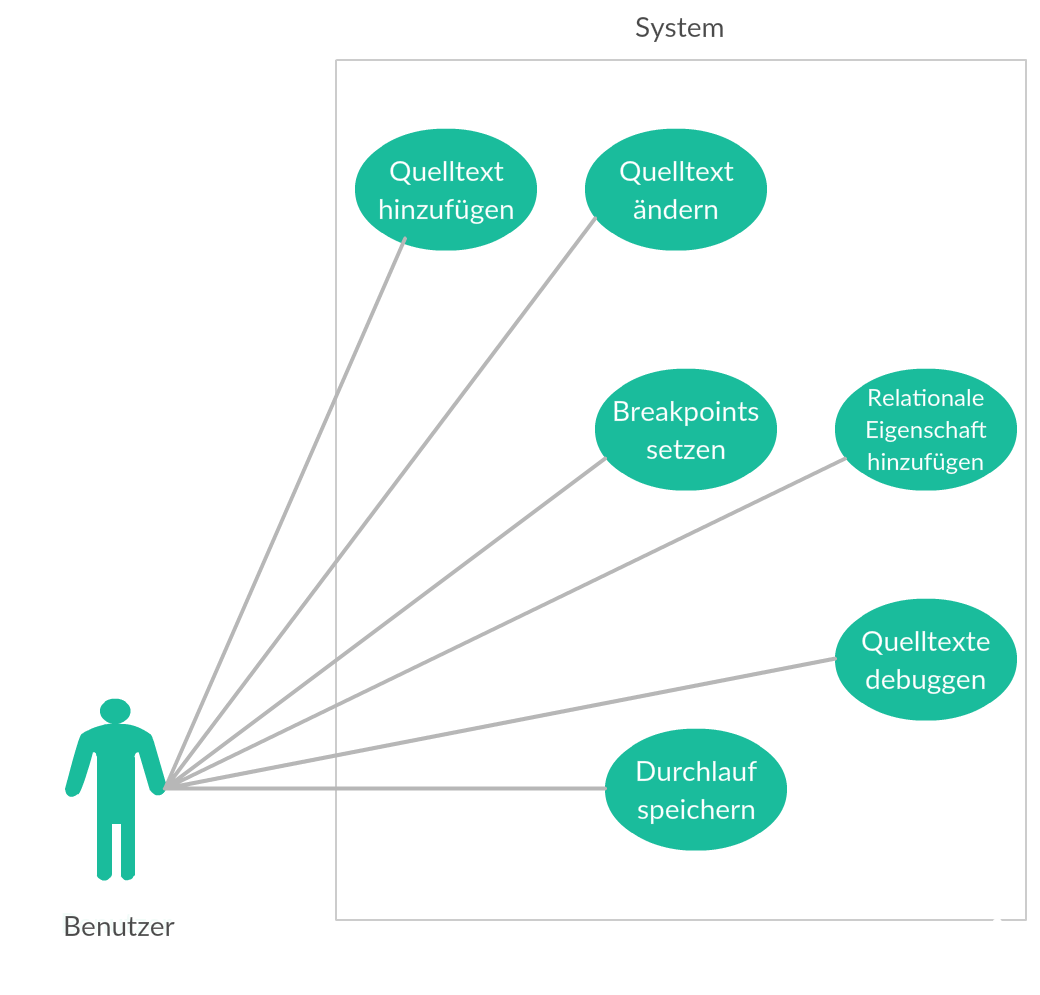
\includegraphics[width=0.7\textwidth]{Anwendungsfalldiagramm}
  \caption{Anwendungsfalldiagramm}
  \label{fig:Bild1}
\end{figure}

In allen Anwendungsfällen ist der Benutzer der einzige Akteur.

\begin{itemize}
		\item[/AF10/] Code hinzufügen: \\ ...
		\item[/AF20/] Code ändern: \\ ...
		\item[/AF30/] Breakpoints setzen: \\...
		\item[/AF40/] Relationale Eigenschaften hinzufügen: \\...
		\item[/AF50/] Codes debuggen: \\
				Die Nutzerin möchte zwei (oder mehr) Programmteile auf relationale Eigenschaften (z.B. Nicht-Interferenz oder Äquivalenz) untersuchen. Dazu fügt sie die zu untersuchenden Quelltexte in das Programm ein, setzt \glspl{Breakpoint} an relevanten Stellen und prüft ihre Annahmen, wo die Programme sich unterscheiden könnten, mit Hilfe von \glspl{Watch-Expression} oder \glsplgen{bedingter Breakpoint}. Ggf. verändert sie den Quelltext ihrer Programme noch einmal. Dann startet sie den \gls{Debugger}. Dieser läuft automatisch bis zum ersten (bedingten) \gls{Breakpoint} durch. Die Nutzerin hat dann die Möglichkeit pro Zeile(n) oder pro Breakpoint vorzugehen. Nach jedem Weitergehen werden ihr die Ergebnisse der Variablen und der Auswertung der \glspl{Watch-Expression} angezeigt. Am Ende des Debug-Vorgangs werden ihr die Ausgabewerte aller Programme angezeigt.
		\item[/AF60/] Durchlauf speichern: \\ ...

\end{itemize}

\section{Globale Testfälle}

\subsection{Basisfunktionen}

\begin{itemize}
	\item[/XX/] Öffnen des Programms
	%\begin{itemize}
	%	\item Vorher: Desktop oder Terminal des Betriebssystems
	%	\item Aktion: Aufrufen des Produkts über Icon oder Terminal
	%	\item Nachher: Produkt öffnet sich in der Default-Ansicht.
	%	\frage{Öffnet das Produkt sich in Default? Wie sieht das aus?}
	%\end{itemize}
	
	\item[/XX/] Öffnen einer Textdatei
	%\begin{itemize}
	%	\item Vorher: \\
	%	Das Programm befindet sich im Editier-Modus und ... \\
	%%	b) es ist noch kein Quelltext geöffnet. \\
		%c) 
		%\item Aktion: Aufruf des File-Chooser-Dialogs im Menüpunkt \enquote{Datei}.
		%\item Nachher: Die ausgewählte Text-Datei
		%\\
		%\frage{Ist das im Editiermodus möglich? Öffnet es sich automatisch in ein neues Textfenster? Welche %Dateiformate sind zugelassen?}
	%\end{itemize}	

	\item[/XX/] Öffnen des Produkts
	\item[/XX/] Öffnen einer Textdatei
	\item[/XX/] Öffnen einer Konfiguration
	\item[/XX/] Speichern einer Konfiguration
	
	\end{itemize}

\subsection{Grundsätzliche Debug-Funktionen}

\begin{itemize}

	\item[/XX/] Setzen eines Breakpoints synchron in allen Textfenstern
	\item[/XX/] Löschen eines Breakpoints in einem Textfenster
	\item[/XX/] Löschen aller Breakpoints eines Fensters
	\item[/XX/] Starten des Debug-Modus
	\item[/XX/] Abbrechen des Debug-Modus
	\item[/XX/] Halten des Debuggers an (bedingten) Breakpoints
	\item[/XX/] Verändern der Schrittlänge.
	\item[/XX/] Einen Schritt der gewählten Schrittlänge in allen Fenstern machen
	\item[/XX/] Einen Schritt der gewählten Länge in einem einzelnen Fenster machen.
	\item[/XX/] Mittels Step-Over eine Funktion nicht inspizieren
	\item[/XX/] Mittels Step-Out aus einer Funktion zurückkehren
	\item[/XX/] Korrektes Ausgeben der Ausgabewerte
	\item[/XX/] Korrektes Auswerten der Watch-Expressions
	\item[/XX/] Korrektes Anzeigen der Zwischenwerte von Variablen
	
\end{itemize}


\subsection{Watch-Expressions}

\begin{itemize}

	\item[/XX/] Hinzufügen einer Expression
	\item[/XX/] Löschen einer Expression
	\item[/XX/] Bearbeiten einer Expression
	\item[/XX/] Hinzufügen einer Markierung
	\item[/XX/] Löschen einer Markierung
	\item[/XX/] Anzeigen einer Markierung
		
\end{itemize}

\subsection{Bedingte Breakpoints}

Siehe Watch-Expressions.


\subsection{Variableneingabe}



\begin{itemize}

\item[/XX/] Angeben des Startwerts einer Variable
\item[/XX/] Angeben einer Wertespanne für den Startwert einer Variablen
\item[/XX/] Einfügen eines zufälligen Startwerts für eine Variable
\end{itemize}

\subsection{Menü-Funktionen}

Ein Item bezeichnet hier jeweils eine Einheit innerhalb eines Submenüs, zum Beispiel eine Watch-Expression innerhalb des Watch-Expression-Blocks oder ein Paar aus einer Variable und ihrem aktuellen Wert in der Variablenausgabe.

\begin{itemize}

	\item[/XX/] Verändern der Item-Reihenfolge
	\item[/XX/] Ein- und Ausblenden von Variablen
	\item[/XX/] Korrektes Anzeigen des Scrollbalkens
\end{itemize}


\newpage
\section{Systemmodelle}
%Architektur, Verhalten, usw
\begin{figure}[h] 
  \centering
     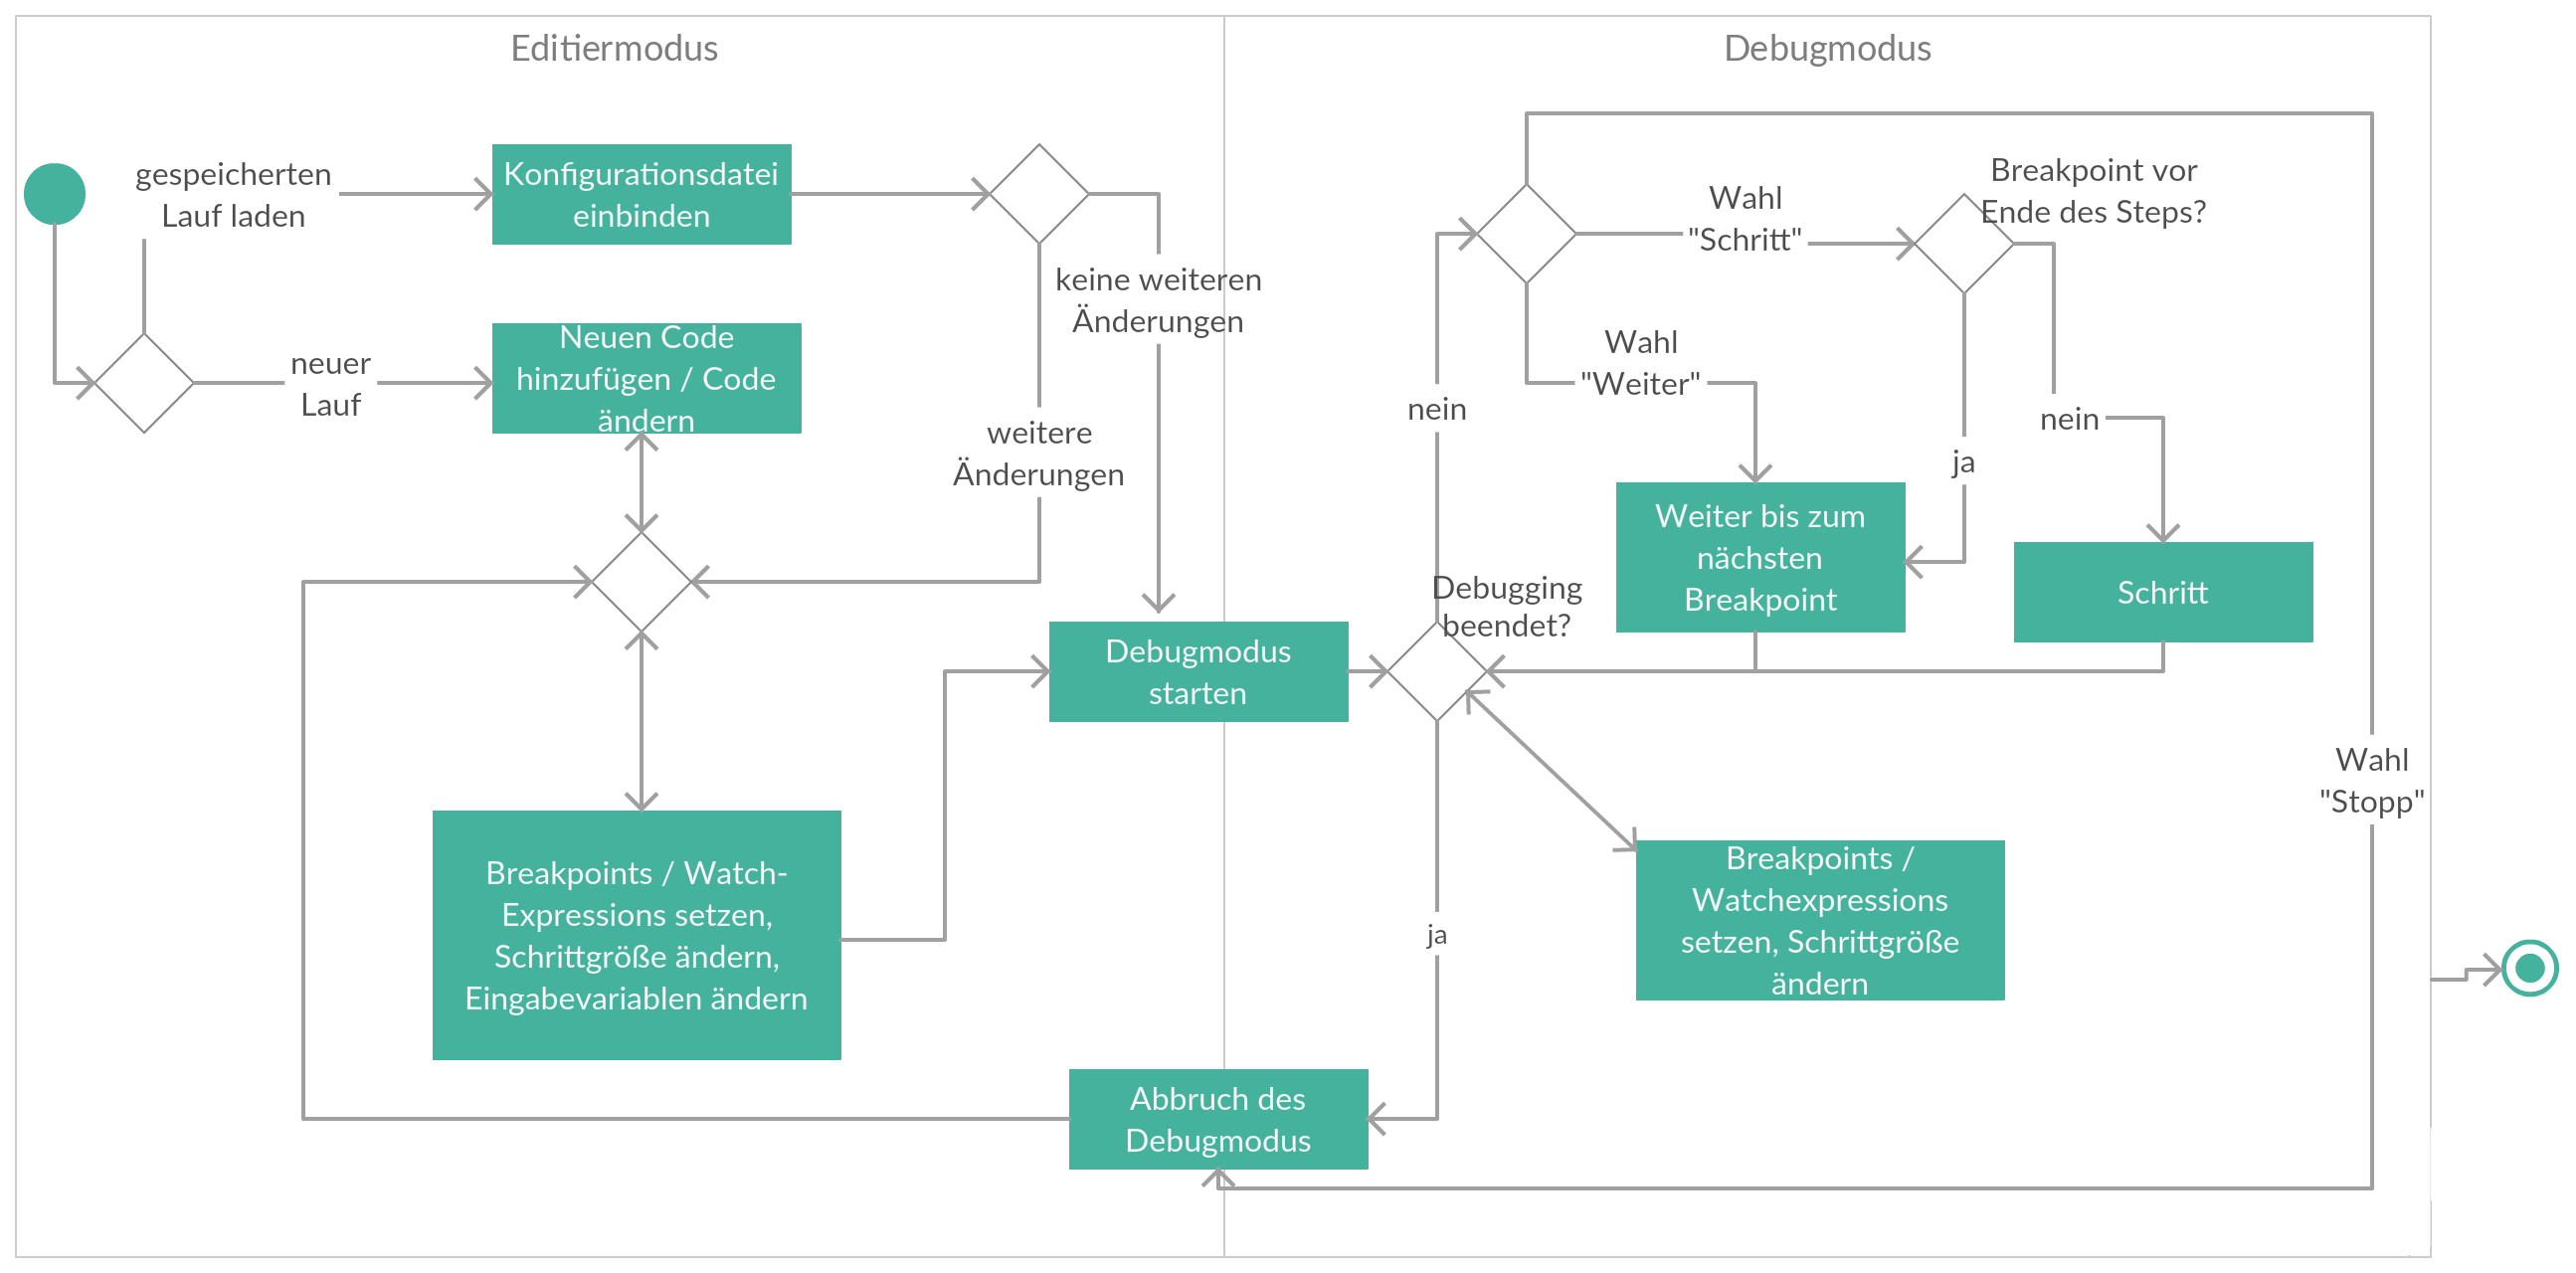
\includegraphics[width=1.0\textwidth]{Aktivitaetsdiagramm}
  \caption{Aktivitätsdiagramm}
  \label{fig:Bild2}
\end{figure}
\vspace{0.7cm}
Das Aktivitätsdiagramm stellt die möglichen Reihenfolgen der Interaktion des Benutzers mit dem Produkt dar. \\
Bindet der Benutzer direkt nach Start des Programms eine \gls{Konfigurationsdatei} eines früheren Laufs ein, kann er diesen Lauf direkt starten, oder vorher Änderungen an den Eingaben und Quelltexten vornehmen. \\
Die Aufteilung in \gls{Editiermodus} und \gls{Debugmodus} zeigt, dass das Ändern und Hinzufügen von Quelltexten und Ändern der Eingabevariablen nicht während des \gls{Debugmodus} möglich sind. Das Ändern von (bedingten) \glspl{Breakpoint}, \glspl{Watch-Expression} und der Schrittgröße ist auch im Debugmodus möglich, allerdings nur zwischen den ausgeführten Schritten und an \glspl{Breakpoint}. \\
Nach manuellem Abbruch oder nach kompletter Durchführung eines Debug-Laufs kehrt das Produkt zum \gls{Editiermodus} zurück. Die vorherigen Eingaben bleiben bestehen, sodass die Wiederholung des Laufs ohne Änderungen direkt möglich ist. Ebenso kann der Benutzer wieder Änderungen an den Eingabevariablen und den Quelltexten vornehmen.\\
Das Beenden des Produkts ist an jeder Stelle möglich.

\newpage

\begin{figure}[!ht]
	\centering
	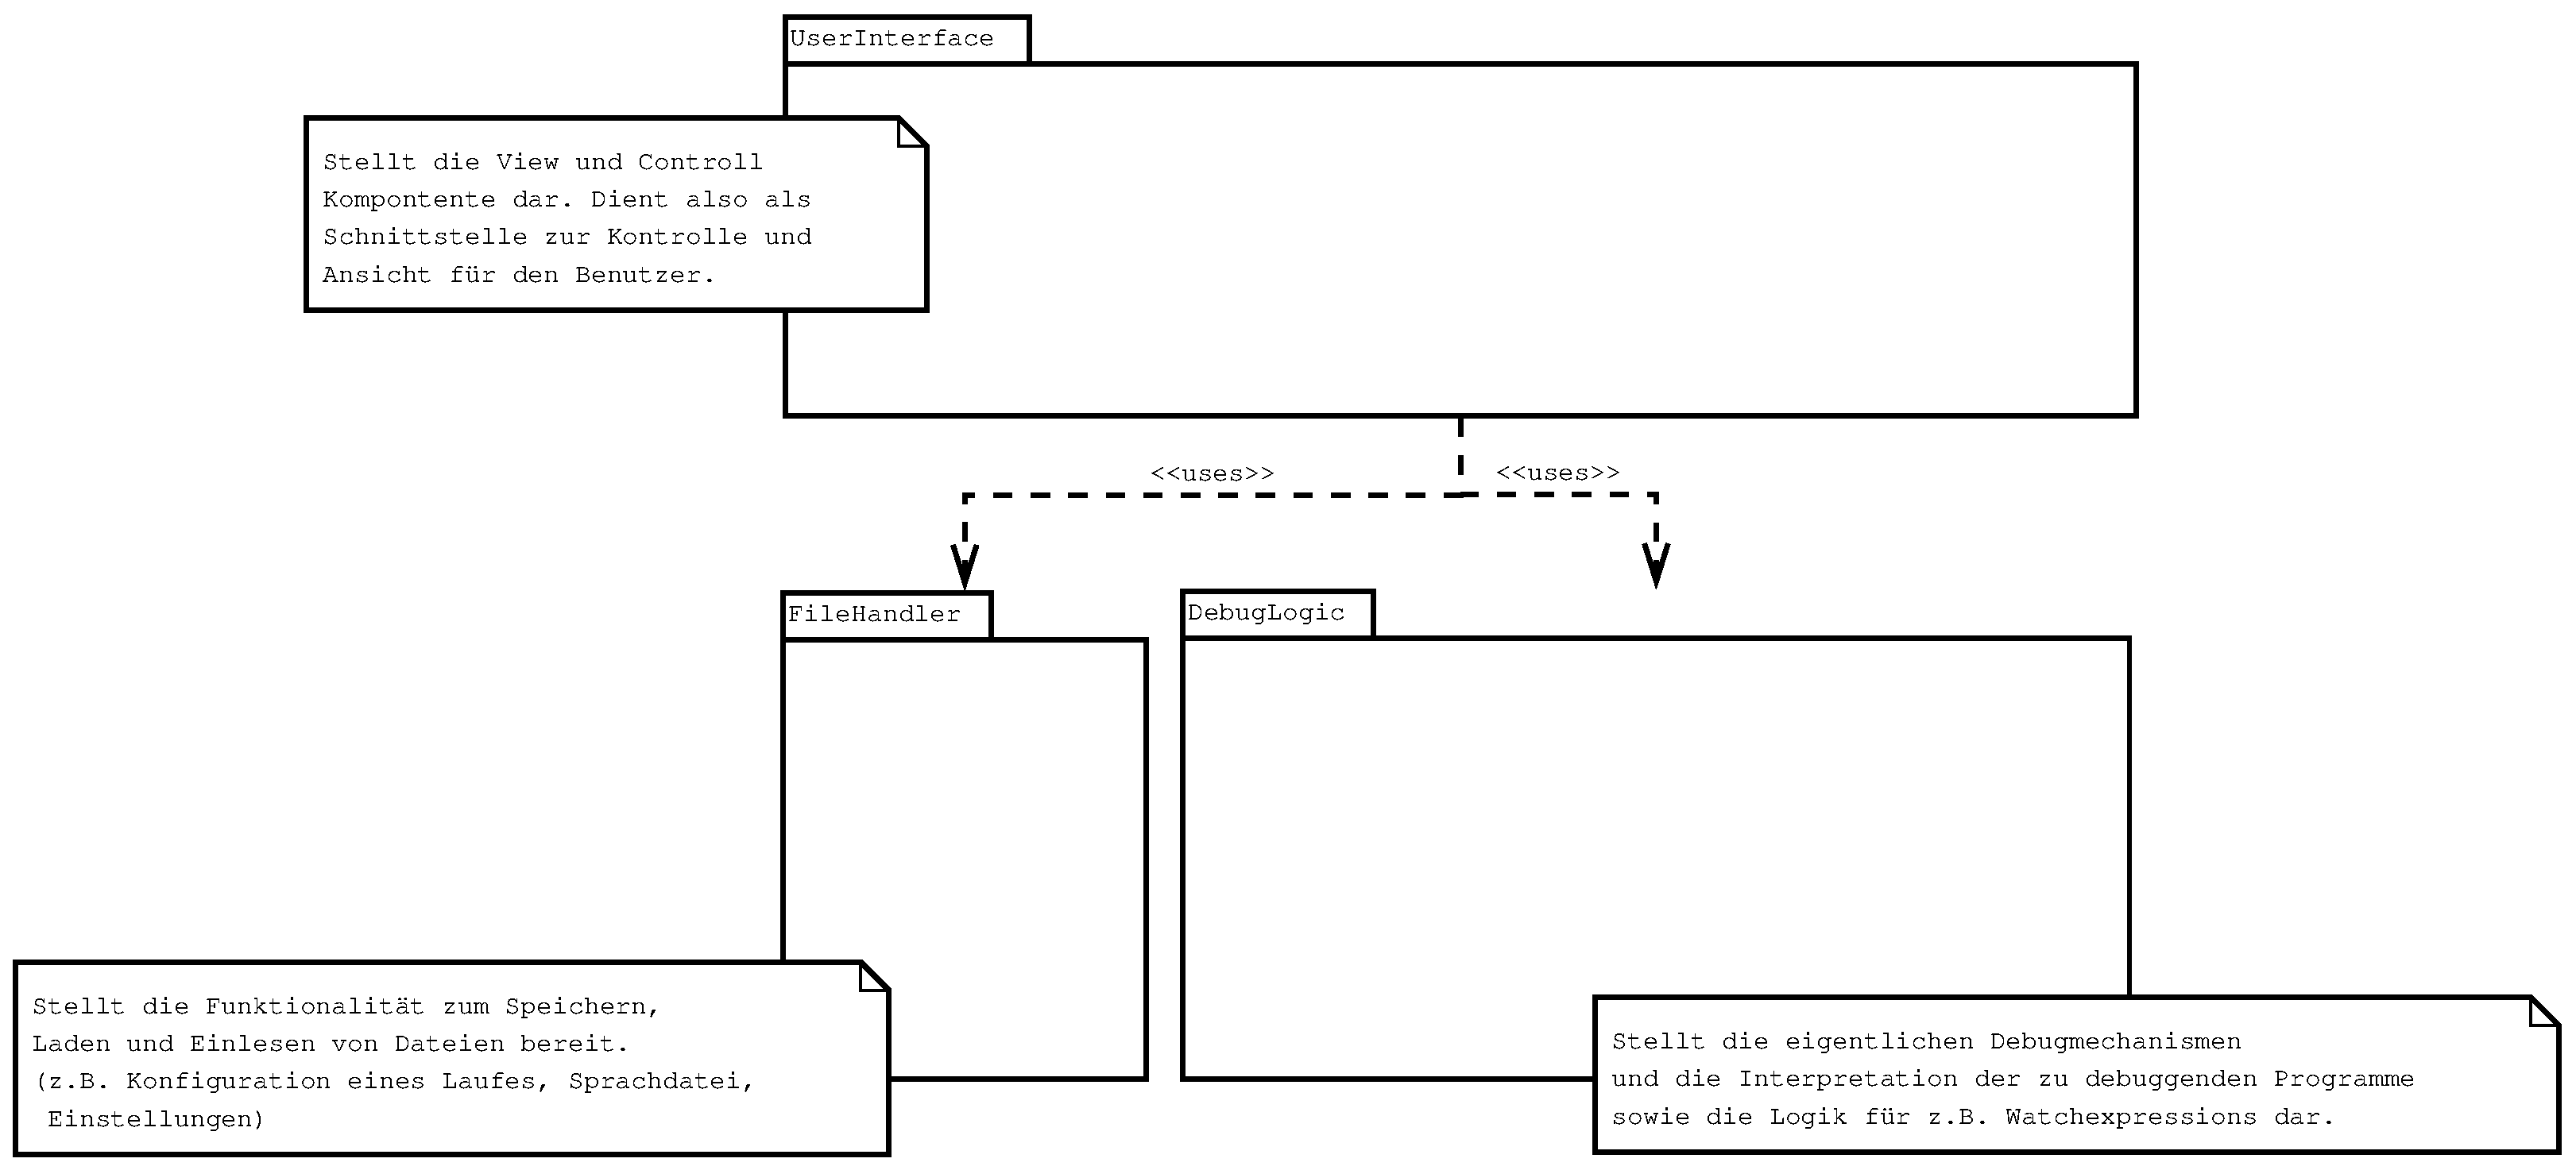
\includegraphics[width=1.0\textwidth]{pakete}
	\caption{Paketdiagramm}
	\label{fig:Bild3} 

\end{figure}
\vspace{0.7cm}
	Während der Definitionsphase ergab sich das obige Paketdiagramm.\\ 
	Diese vorläufige Version des Paketdiagramms wird als Grundlage für den Entwurf des
	Produkts in der Entwurfsphase verwendet.
	
\newpage
\section{Benutzungsoberfläche}
%Gui-Skizzen, Erklärungen der Menüs, usw
\begin{figure}[!ht] 
    \vspace{-10pt}
    \centering
       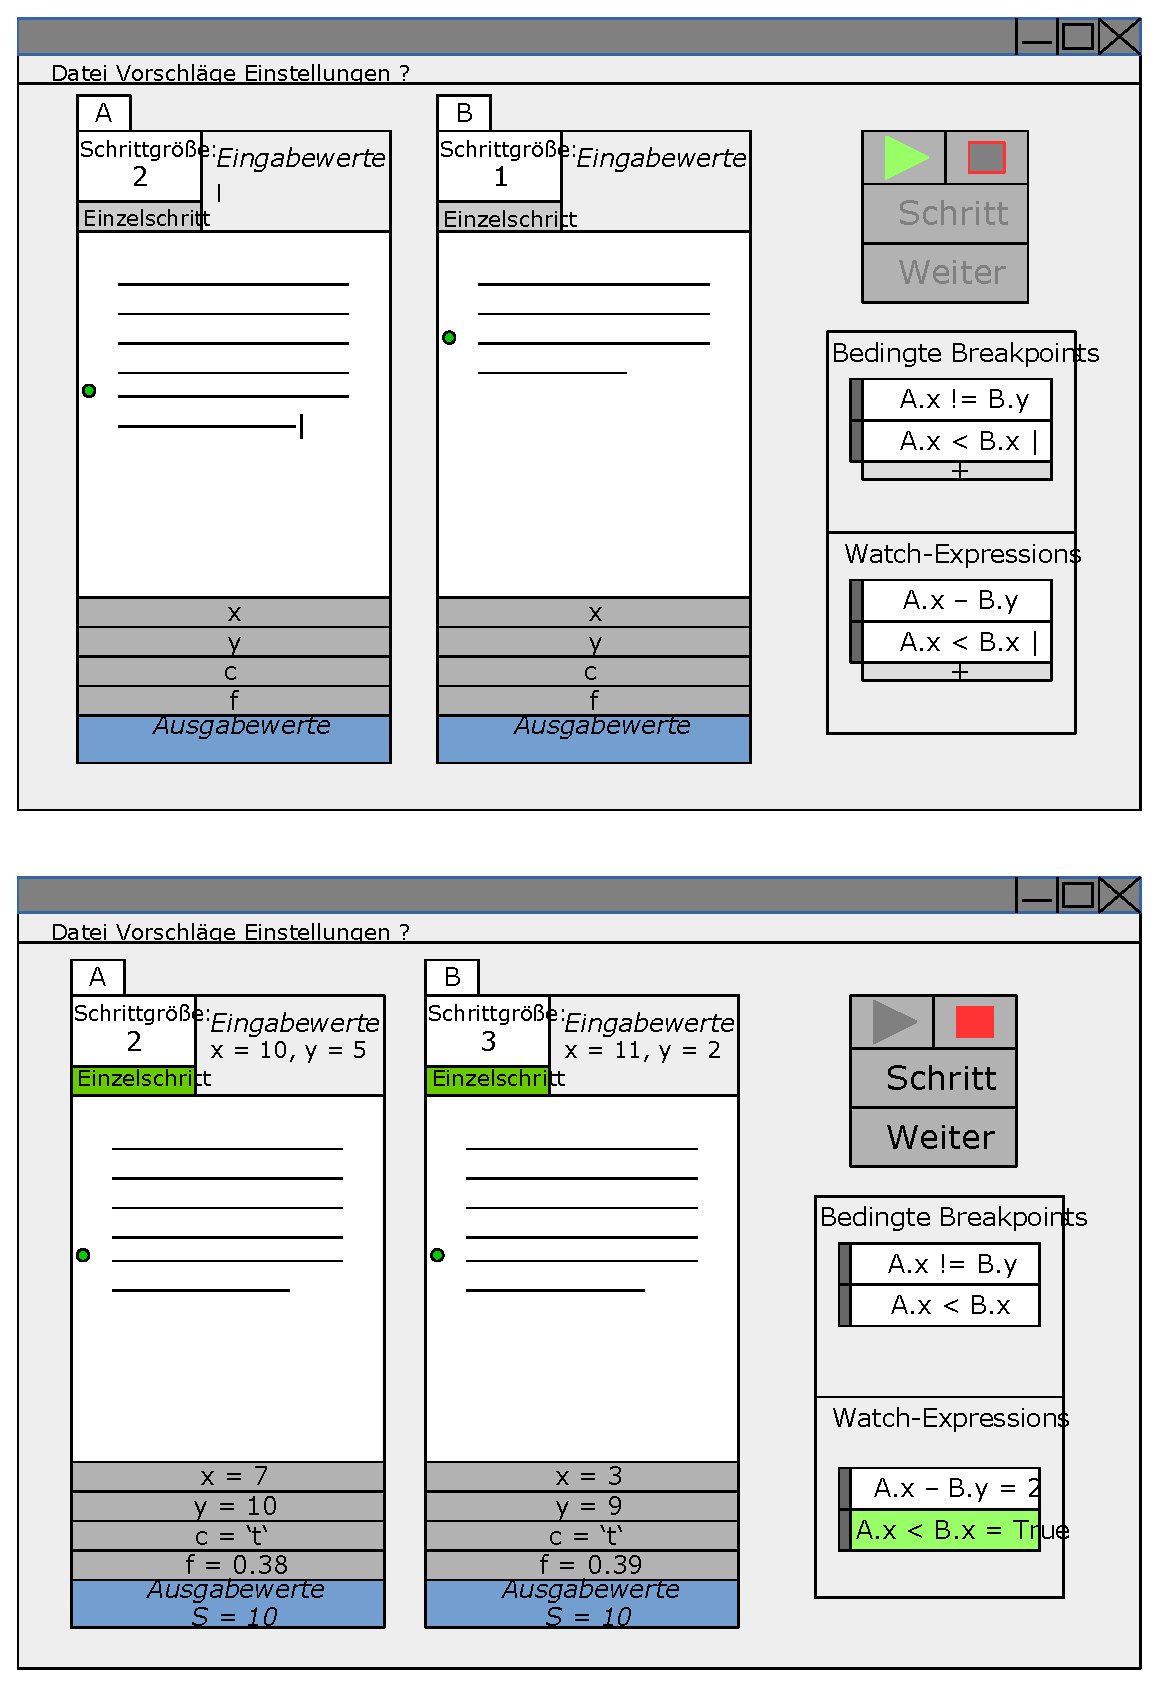
\includegraphics[width=0.87\textwidth]{skizzeFull.eps}
       \caption{
         Benutzeroberfläche des Produktes im Editiermodus (oben) und im Debugmodus
         (unten)
       }
    \label{fig:Bild4}
\end{figure}

\newpage
    \subsection{Beschreibung}
        Befindet sich das Produkt im \gls{Editiermodus}, so können die Eingabequelltexte über die 
        Eingabefenster bearbeitet werden.
        Durch Verändern des Textes im Bereich \enquote{Eingabewerte} können Werte der Eingangsvariablen
        spezifiziert, gelöscht und verändert werden. 
        \glsplcap{bedingter Breakpoint} und \glspl{Watch-Expression} können durch Betätigung der jeweiligen 
        \enquote{+}-Schaltflächen hinzugefügt werden.
        Die Schaltflächen \enquote{Schritt} und \enquote{Weiter}, sowie \enquote{Einzelschritt} können nicht betätigt
        werden. Betätigung der Schaltfläche mit dem grünen Pfeil verursacht den Übergang von
        das Produkt in den Debugmodus.
        
        Befindet sich das Produkt im \gls{Debugmodus}, können die Eingabequelltexte nicht
        über die Eingabefenster bearbeitet werden. Die \enquote{+}-Schaltflächen für bedingte Haltepunkte
        und \glspl{Watch-Expression} können nicht betätigt werden.
        Die Schaltflächen \enquote{Schritt}, \enquote{Weiter} und \enquote{Einzelschritt} können betätigt werden.
        Betätigung der Schaltfläche mit dem roten Viereck verursacht den Übergang von --Programmname-- in den Editiermodus.
        
\section{Anforderungen an die Entwicklungsumgebung}
Bei der Erstellung des Aktivitäts- und Anwendungsfalldiagramms wurde die Freie Version des Online-Diagramm-Editors \href{https://creately.com/}{Creately} verwendet.\\
Das Produkt wird in Java entwickelt. Dazu werden die Java-Entwicklungsumgebungen IntelliJ\textsuperscript{\textcopyright} und Eclipse\textsuperscript{\textcopyright} verwendet.\\
\newpage
        
\section{Zeit- und Ressourcenplanung}
% Tabelle mit Phasendaten (Ideen sammeln, Einzelarbeit, Ideen zusammentragen, Überarbeitung, Abgabe Vorversion, Kolloquium/Abgabe Finalversion)
\subsection{Zeitliche Gesamtplanung}
\textit{06.11.2017 - 26.11.2017} Definitionssphase \\
\textit{27.11.2017 - 24.12.2017} Entwurfsphase \\
\textit{08.01.2018 - 04.02.2018} Implementierungsphase\\
\textit{19.02.2018 - 11.03.2018} Qualitätssicherungsphase\\
\textit{12.03.2018 - 25.03-2018} Abnahme und Präsentation

\subsection{Phasenverantwortliche:}
Definitionsphase: Chiara Staudenmaier\\
Entwurfsphase: Joana Plewnia, Benedikt Wagner\\
Implementierungsphase: Pascal Zwick\\
Qualitätssicherungsphase: Etienne Brunner\\
Präsentation/Abnahme: Ulla Scheler\\

\subsection{Vorraussichtliche zeitliche Feinplanung}
\subsubsection{Definitionsphase}
\textit{bis 06.11.} Sammeln der Inhalte\\
\textit{bis 13.11.} Formulierung der Punkte im Pflichtenheft in Einzelarbeit\\
\textit{bis 17.11.} Gemeinsame Überarbeitung\\
\textit{17.11. 11:30 Uhr} Abgabe der vor-finalen Version des Pflichtenhefts\\
\textit{bis 24.11.} Gemeinsame Überarbeitung\\
\textit{24.11. 11:30 Uhr} Abgabe der finalen Version des Pflichtenhefts \\

\subsubsection{Entwurfsphase}
\textit{bis 03.12.} Fertigstellung der Einteilung des Systems in Pakete und Unterpakete und Festlegung der Schnittstellen derer. \\
\textit{bis 10.12.} Fertigstellung der Einteilung der Pakete in Klassen und definieren der Methoden und Attribute derer \\
\textit{bis 17.12.} Fertigstellung der Paket- und Klassenbeschreibungen und des vorläufigen Entwurfsdokumentes\\
\textit{22.12.} Abgabe des endgültigen Entwurfs. 

\subsubsection{Implementierungsphase}
\textit{bis 14.01.} Fertigstellung der Dateiverwalter und des Interpreters. Beginn an Front- und Backend.\\
\textit{bis 21.01.} Fertige, aber noch nicht funktionelle Benutzeroberfläche. Bereitstellung einiger Methoden des Backends für diese.\\
\textit{bis 28.01.} Vollständige Implementierung des Backends und ein funktionierendes Frontend.\\
\textit{bis 04.02.} Ende und Abgabe der Implementierung des Programms.

\subsubsection{Qualitätssicherungsphase}

\subsubsection{Abnahme und Präsentation }
\textit{bis 16.03.} Einarbeiten der Anmerkungen aus dem letzten Kolloquium \\
\textit{bis NN} Anfertigung der Abschlusspräsentation

\section{Ergänzungen}
%Sprache
\subsection{Sprache}
Die Programmiersprache, in der die zu debuggenden Programme verfasst sind, wird im Folgenden als die Sprache bezeichnet. 
\paragraph{Klassifikation der Sprache} Die Sprache ist prozedural und imperativ, nicht objektorientiert und nicht einrückungsbasiert.
\paragraph{Elemente der Sprache}
Die Sprache unterstützt die folgenden primitiven Datentypen:
\begin{itemize}
\item  32-bit Ganzzahlen: \texttt{int}
  \item  64-bit Ganzzahlen: \texttt{long}
 \item  32-bit IEEE 754 Fließkommazahlen: \texttt{float}
 \item   64-bit IEEE 754 Fließkommazahlen: \texttt{double}
  \item  Einzelnes Zeichen: \texttt{char}
  \item  Wahrheitswert: \texttt{boolean}
\end{itemize}
Zudem sind bis zu dreidimensionale Arrays dieser Datentypen möglich.
Ferner unterstützt die Sprache die folgenden Kontrollstrukturen:
\begin{itemize}
\item Funktionen und Prozeduren, also Unterprogramme mit oder ohne Rückgabewert.
\item Bedingte Ausführung: \texttt{if, else if, else}
\item Schleifen: \texttt{while}
\end{itemize}
Es muss in jedem Programm eine \texttt{main}-Routine vorhanden sein, von der die Ausführung ausgeht. Routinen, die aufgerufen werden, müssen darüber stehen. Kommentare können sowohl zeilenweise (\texttt{//}) als auch zeilenübergreifend (\texttt{/*Kommentar*/}) benutzt werden. Sämtliche Variablen müssen innerhalb einer Routine stehen. Auch Rekursion ist möglich.
\newpage

\paragraph{Syntax der Sprache}
Die Syntax der Sprache ist angeleht an gängige Sprachen wie C oder Java. Im folgenden Listing ist ein Beispielprogramm aufgeführt. 

\begin{verbatim}
void doSenselessStuff() { //Prozedur ohne Rückgabe
    int a = 0;
}
float devide(float x, float y) { //Funktion mit Rückgabewert
    if(y != 0)	
        return x/y;
    return -1; //Rückgabe
}
int main(int j, int k)
{
    int a; //Deklaration
    a = 1; //Zuweisung
    long x = 100000L; 
    int b = 2; // Deklaration mit Initialisierung
    int[j+k] myInts; \\Arraydeklaration
    char[8] myChars= {'a','b','c','d'};
    if(j<k) {
        int i = 0;
        while(i<j) {
            myInts[i] = 0; //Arrayzugriff
            i=i+1;
        }	
    } else if(j==k) {
        return 0;
    } else
        return -1;
    doSenselessStuff(); //Routinenaufruf
    float z = devide(3.0f*k /1.1f);
    return z+j;
}
\end{verbatim}
\newpage
\subsection{Syntax bedingter Breakpoints und der Watch-Expressions}
Die Syntax der Watch-Expressions und bedingten Breakpoints ist durch folgende kontextfreie Ableitungsregeln gegeben: \\\\
<WatchExpression> $\rightarrow$ <BooleanExpression> | <Term>\\\\
<BedingterBreakpoint> $\rightarrow$ <BooleanExpression>\\\\<BooleanExpression> $\rightarrow$ <Term> < <Term> 
| <Term> > <Term> |\\ <Term> >= <Term>|<Term> <= <Term>| <Term> == <Term>| \\<Term> != <Term>\\\\
<Term> $\rightarrow$ <Term> / <Term> 
| <Term> * <Term> |\\ <Term> - <Term>|<Term> + <Term>| <Atom>\\\\

Wobei ein <Atom> ein fester Wert eines Datentyps (z.B. \texttt{5, 'c', true}) oder eine Variable der Form <Programmbezeichner>.<Variablenname> (z.B. \texttt{A.x} für Variable x in Programm A) ist. \\
Das heißt, Watch-Expressions werten sich zu einem beliebigen Wert aus, während sich bedingte Breakpoints immer zu einem Wahrheitswert auswerten.


\newpage
\printglossary[style=altlist,title=Glossar]



\end{document}
\grid
